\documentclass[twocolumn,aps,prb,citeautoscript]{revtex4-1}
\usepackage{graphicx,amsmath,amssymb}

\begin{document}

\title{SURF Progress Report 2:\\
Effects of a superconducting lead endcap \\ on the magnetic field
profile for the nEDM search}
\author{Aritra Biswas, with Filippone Group}
\affiliation{Kellogg Radiation
Laboratory, California Institute of Technology}

%\begin{abstract}

%\end{abstract}

\maketitle

\section{Motivation}

\subsection{Group goal: the half-scale model}

The discovery of charge-parity symmetry (CP) violation 
in the decay of neutral kaons has inspired attempts to extend the
Standard Model \cite{cpv}. Measurement of a non-zero electric dipole
moment (EDM) in the neutron would be another instance of CP violation that
could guide these attempts and help confirm predictions about the asymmetry of
matter and antimatter in the universe.

The neutron electric dipole moment (nEDM) collaboration intends to
improve \cite{krl} the currently-measured limit \cite{ill}
on the neutron EDM with new experimental techniques.
Trapped ultra-cold neutrons (UCN) precess in the presence
of a constant magnetic field or a variable electric field. Measuring
a change in precession correlated with the electric field
would confirm a non-zero EDM.

An important obstacle is eliminating a ``geometric phase effect''
that creates a shift in the UCN precession and results in
a false EDM reading. Since this effect is caused by field gradients,
we need to make the magnetic field as uniform as possible.
To tackle this engineering challenge,
we have constructed a half-scale model of the magnet that will be
used in the nEDM experiment. We are simulating and measuring
the effects of various types of shielding ($\mu$-metal,
ferromagnetic Metglas, and superconducting lead) in order to
determine the optimal magnet design, with the desired field uniformity,
for the nEDM experiment.

\subsection{SURF goal: superconducting endcaps}

The current half-scale model (fig. \ref{fig:structure})
features a cylindrical $\cos\theta$ coil \cite{coil} (referred to as the $B_0$ coil)
surrounded by concentric open-ended cylindrical shells for shielding.
In order to improve field uniformity, we investigate the effects of superconducting
lead endcaps to close the open ends of the cylindrical axial lead shield.

%Since November 2013 (when I first stared work in this group), we have designed and installed
%a bottom endcap. Measurements taken afterwards suggested that a top endcap would be more
%effective.

As of August 2014, we have installed an endcap covering the top $(z>0)$ opening
of the lead shield, and have cooled this
endcap to a superconducting state twice. Analysis of resulting data is ongoing.

The goal of this SURF is to help develop a reliable simulation of
this endcap, measure its effects, explain any inconsistencies, and determine how effective
this endcap style will be for the final nEDM experiment.

\begin{figure}
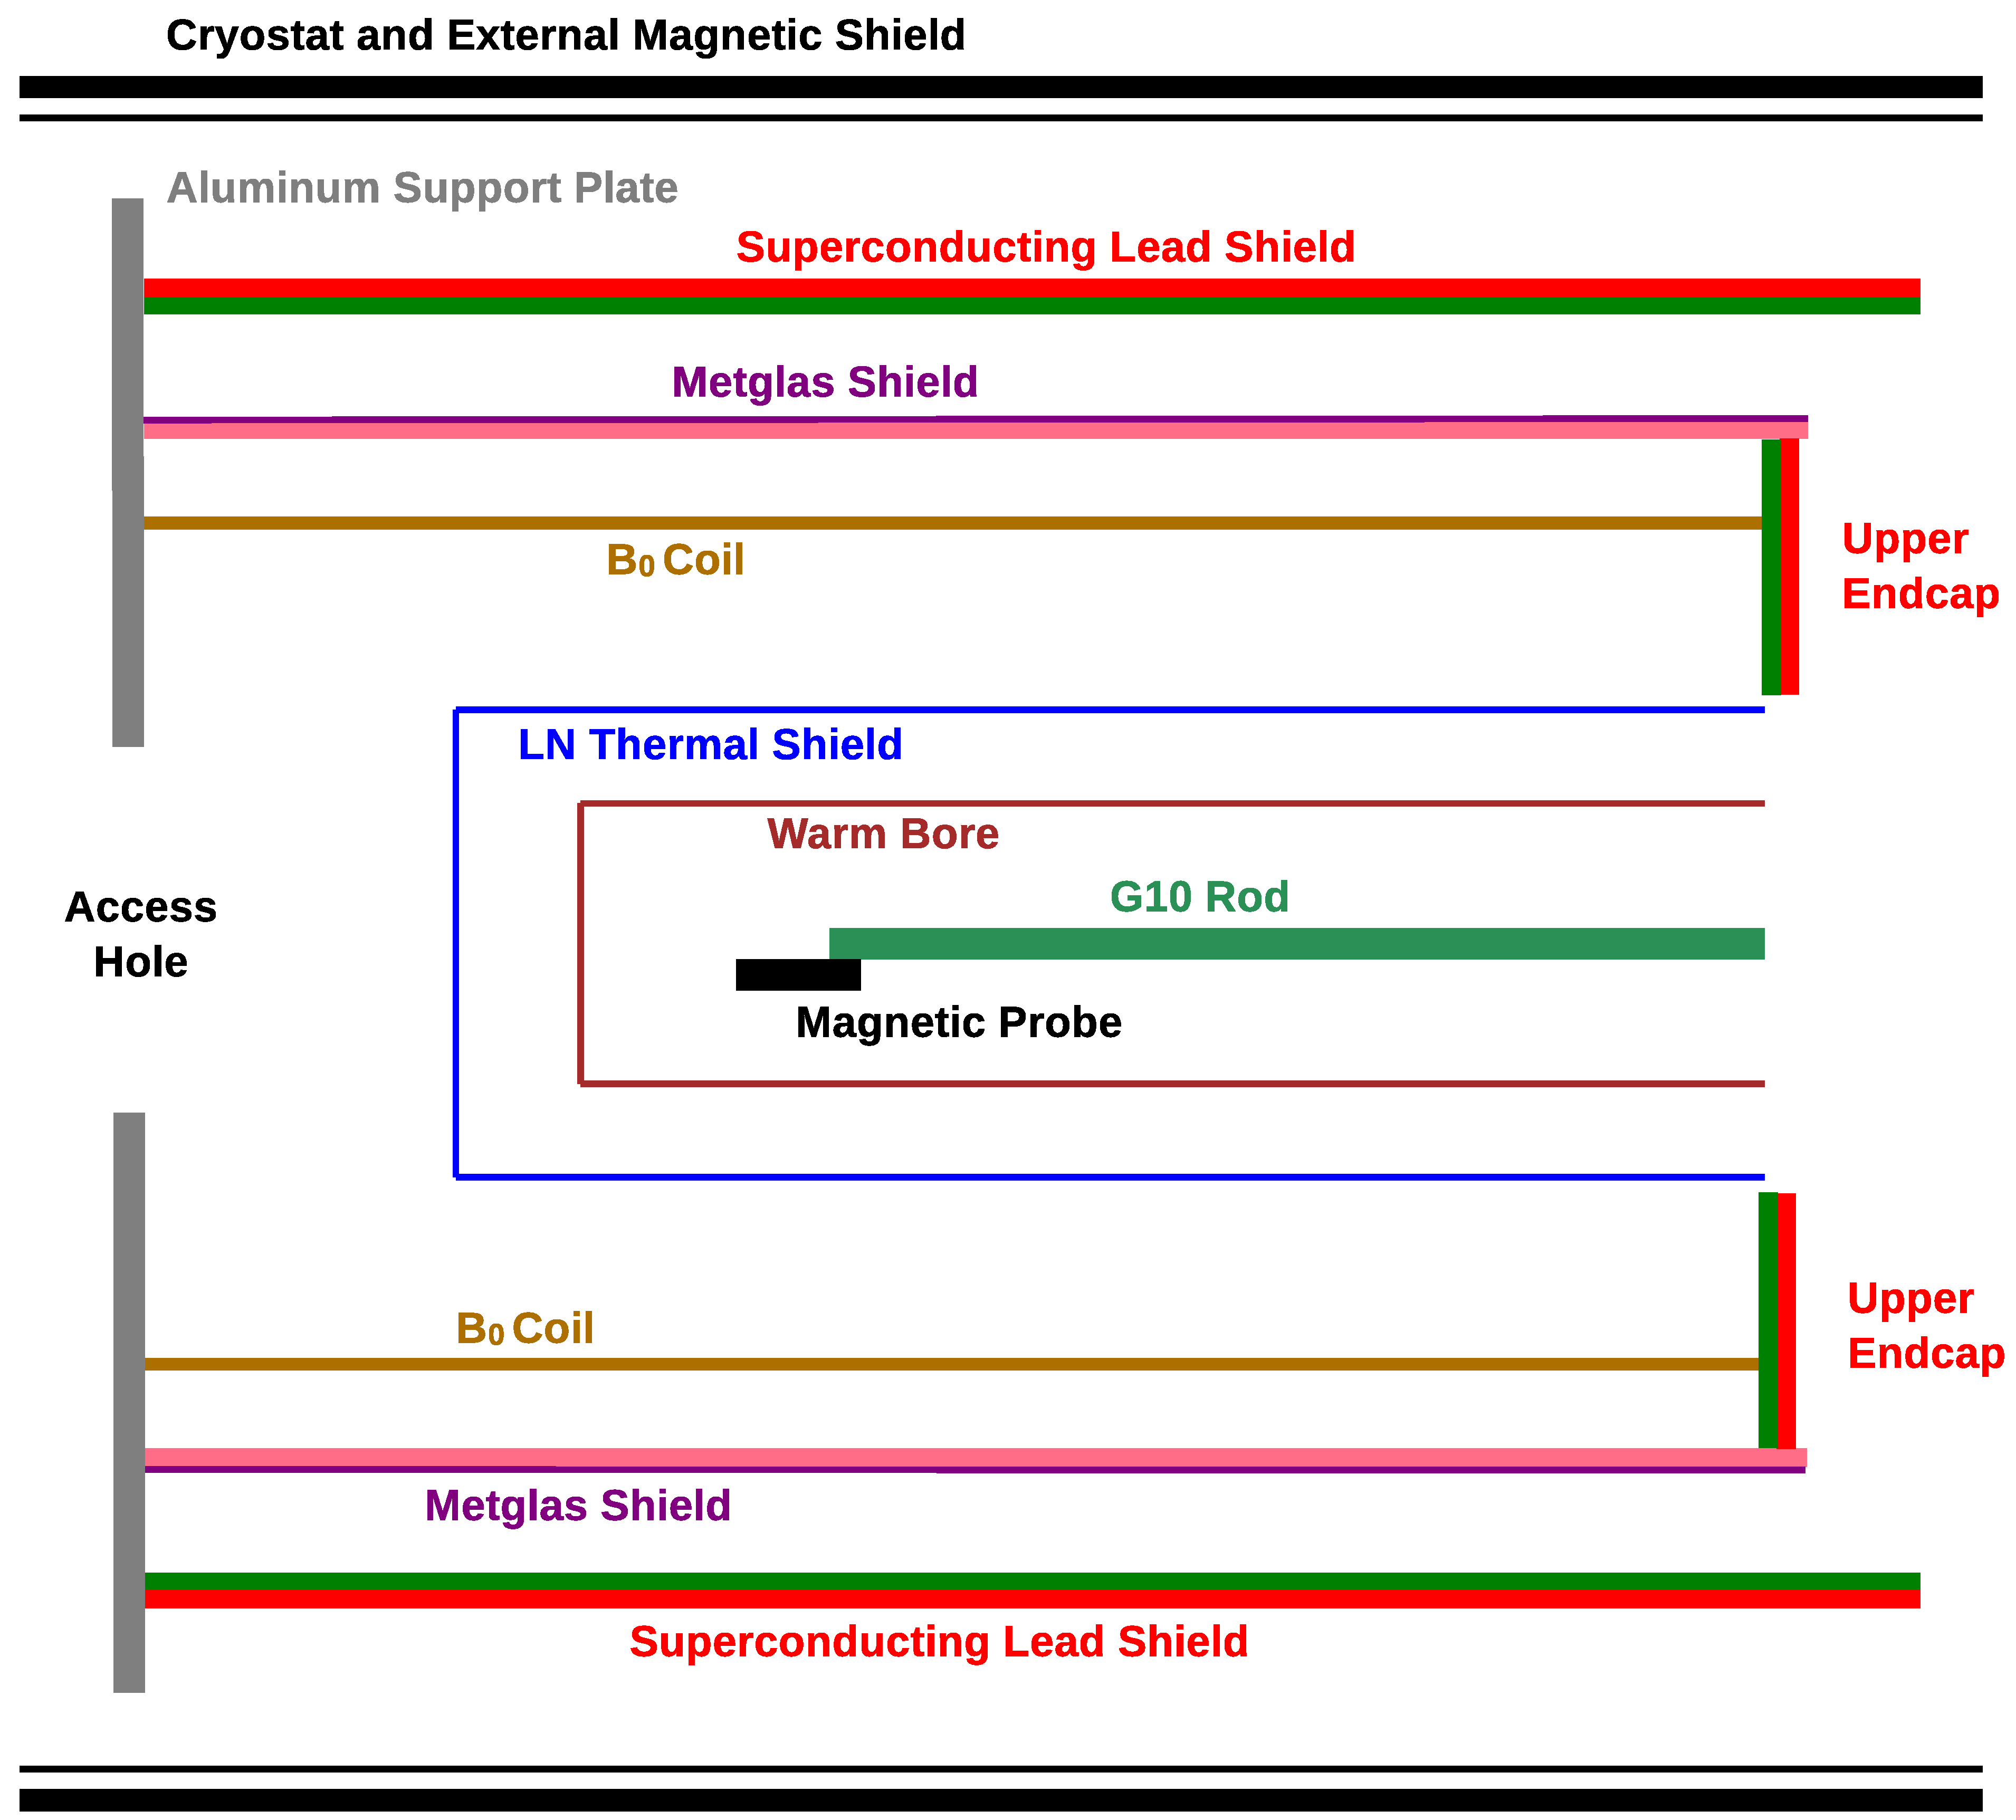
\includegraphics[angle=90, width=0.45\textwidth]{figures/structure.eps}
\caption{\label{fig:structure}Stylized diagram of the experimental
setup.}
\end{figure}

\section{Data collection procedures}

\subsection{Tools developed for this project}

I have developed various programs to streamline the collection and analysis of data.
We use National Instruments Labview to interface with temperature sensors, magnetic probes, shimming coils,
and other apparatus in the lab. Creating a detailed map of the magnetic field often takes several hours,
and the external magnetic field
can change dramatically during this time; for example, we have had abberations in our data because a truck
parked outside the lab. To avoid this issue, I created a program to monitor the external field at various
locations, allowing us to know when the external field has changed dramatically and to throw out data accordingly.

I have also created a specialized plotting program (currently 468 single lines of code) to analyze
our field maps, apply various corrections, and compare them with simulations.

\subsection{Analysis process and corrections}

We are using \texttt{RotationShield}, a ``linear matrix solver for systems with cyclic symmetry'' developed previously in the group, \cite{rotshield}
to simulate our magnet and predict the effects of the superconducting endcap. Before comparing measured field maps
to results from these simulations, several corrections must be applied.

\subsubsection{Background subtraction}

For each map, we must measure the background magnetic field (i.e. when the $B_0$ coil is turned off) and
subtract this field from the foreground ($B_0$ on). This step allows us to isolate the effects of our changes in
shielding geometry.

\subsubsection{Probe centering}

We have found that the field profile is highly sensitive to $x$ position. For example, along the cylinder's
central axis ($x=0, y=0$), simulations predict that $B_z$ should be 0; however, when $x\neq0$,
the $B_z$ vs. $z$ curve exhibits
a peak near $z=1.073$ m, the end of the $B_0$ coil. The height of this peak is directly correlated with the $x$
position. Early comparisons showed a $B_z$ vs. $z$ peak even along $x=0, y=0$, and measurements confirmed that
the probe setup is not correctly centered along the $x$ axis. Since such centering is difficult, we measure the
offset and correct for it during data analysis. For example, data taken along $x = 0.1$ m, after correction,
is recognized as data taken along $x = 0.104$ m, so we can compare the curve to the appropriate simulated curve.

\subsubsection{Probe offset}

Our magnetic probe is composed of three separate one-axis probes which are separated along the $z$-axis.
The probe's location corresponds to the location of the $B_z$ probe specifically. This means that when the probe is
at $(0, 0, 0)$, the $B_x$ probe, for example, is actually at $(0, 0, 0.015\text{ m})$. The data that we collect
cannot be expressed as a single vector map, then, since we are not guaranteed to have a vector $(B_x, B_y, B_z)$
for every point $(x, y, z)$. In the analysis program, I work around this by implementing an \texttt{OffsetAxis}
class which, for each spatial axis, is capable of storing an offset vector corresponding to the components
of the field. Thus, the $z$ axis can be offset depending on whether we are graphing $B_x$ vs. $z$ or
$B_z$ vs. $z$.

\subsubsection{Probe tilt}

The probe's rigid mount introduces another problem: the probe cannot be perfectly vertical.
Since $B_x >> B_z$ at
magnet center, even a very small angle can make the $B_z$ probe pick up part of the $B_x$ signal;
this effect is illustrated in
Figure \ref{fig:angle}. The probe, tilted at some angle $\theta$, gives skewed readings $B_x'$ and $B_z'$.

\begin{figure}
\vspace{15pt}
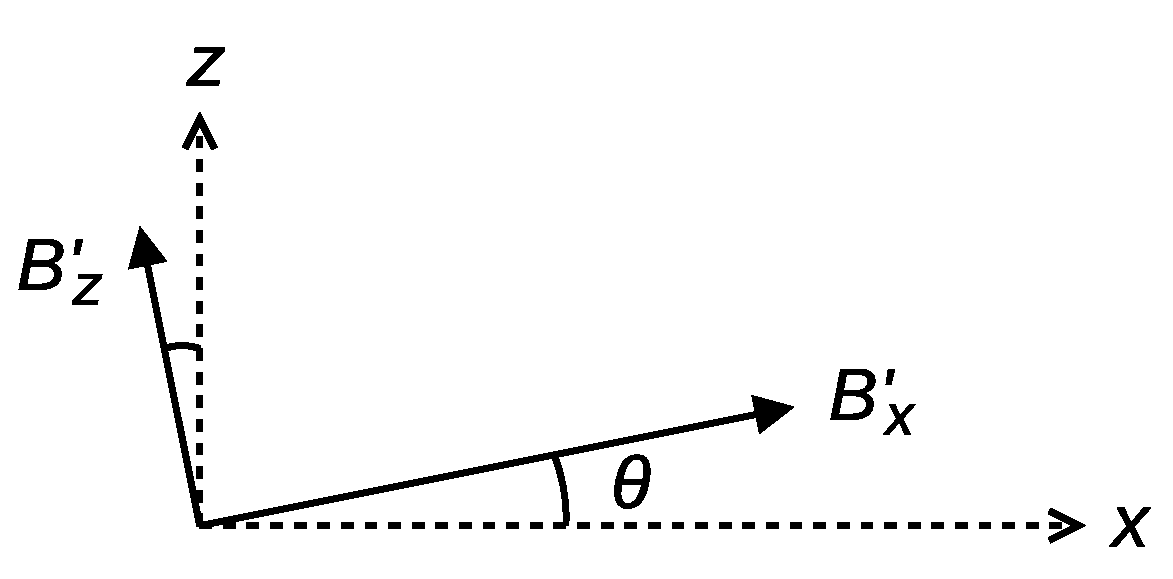
\includegraphics[width=0.45\textwidth]{figures/probe_tilt.eps}
\caption{\label{fig:angle} A diagram of the probe tilt. The $x$ and $z$ axes are correct relative
to the magnet. However, because the probe is tilted at some angle $\theta$, the given $B_x'$ and $B_z'$
are misaligned.}
\end{figure}

Knowing $\theta$, we could find the correct $B_x$ and $B_z$:

\begin{align*}
B_x &= B'_x \cos\theta - B'_z \sin\theta \\
B_z &= B_z' \cos\theta + B_x' \sin\theta
\end{align*}

To find $\theta$, we use the knowledge that $\theta$ is small and that, at magnet center,
$B_z$ should be 0:

\begin{align*}
B_x &= B'_x - B'_z \theta \\ B_z &= B_z' + B_x' \theta \\
\theta &= -\frac{B'_z}{B'_x}.
\end{align*}

We thus find $\theta$ using measurements of $B_x'$ and $B_z'$ near magnet center, then apply the
correction everywhere.

\subsubsection{Normalization}

Simulation output from \texttt{RotationShield} gives the magnetic field in arbitrary units, so the expected
magnetic field strength at any location is known only relative to another known location. To compare these simulations
with our measured output, I draw a small cube around magnet center $(0, 0, 0)$ in the measured map,
calculate the average $B_x$ inside, and normalize the simulated map such that $B_x$ at its center matches the
measured map. This adjustment allows fair comparison of absolute field strengths at any location.

\begin{figure*}
\includegraphics[width=0.9\textwidth]{../savedplots/pr2_agree.eps}
\caption{\label{fig:agree}$B_z$ vs. $z$ along $x = 0.104$ m, $y = 0$. Blue and yellow curves are data and simulation
(respectively) when both the endcap and the axial shield are superconducting; red and black curves are data and
simulation when neither is superconducting.}
\end{figure*}

\section{Observations}

Comparisons of measured maps with simulations in the non-superconducting state allow us to assess the accuracy
of our data collection procedures; these comparisons prompted many of the aforementioned data corrections.

Data from our latest cooldown on August 7 shows good agreement with simulations
in both normal and superconducting cases (see
figure \ref{fig:agree}).

An additional
measurement, with the axial lead shield superconducting and the endcap in an unknown state (call this
configuration A), revealed interesting aspects about the axial shield's effect on the field.
Configuration A data agreed with measurements when both the
axial shield and endcap were non-superconducting (configuration B),
suggesting that the endcap was non-superconducting in configuration A and
that axial lead shield provides a small, almost negligible correction. This is expected since the axial shield
is primarily designed to shield the field from environmental fluctuations, not to enforce field uniformity.

However, further analysis revealed that the axial shield alone can exhibit a strong ``$B_z$ suppression effect''
when it
extends above the Metglas shield, and that the presence of a superconducting endcap effectively hides this effect.
This suggests that the endcap may have been partially superconducting in configuration A, and that the
axial shield geometry is such that its extension above the Metglas shield is minimal. Analysis of this effect
is ongoing.


\begin{thebibliography}{}
\bibitem{cpv} Cronin, J. ``Nobel Lecture: CP Symmetry Violation – The Search
for Its Origin,'' Nobel Media AB (2013).
\bibitem{ill} Baker, C. A., D. D. Doyle, P. Geltenbort, K. Green, M. G. D. Van der Grinten, P. G. Harris, P. Iaydjiev et al. ``Improved experimental limit on the electric dipole moment of the neutron.'' \textit{Physical Review Letters} 97, no. 13 (2006): 131801.
\bibitem{krl} ``Search for the nEDM at Caltech.'' Kellogg Radiation Laboratory
$\langle$krl.caltech.edu$\rangle$ (2014).
\bibitem{endcapstyles} Malkowski, S., R. Y. Adhikari, J. Boissevain, C. Daurer, B. W. Filippone, B. Hona, B. Plaster, D. Woods, and H. Yan. ``Overlap Technique for End-Cap Seals on Cylindrical Magnetic Shields.'' \textit{IEEE Transactions on Magnetics} 49, no. 1 (2013): 651-653.
\bibitem{coil} Perez Galvan, A., B. Plaster, J. Boissevain, R. Carr, B. W. Filippone, M. P. Mendenhall, R. Schmid, R. Alarcon, and S. Balascuta. ``High uniformity magnetic coil for search of neutron electric dipole moment.'' \textit{Nuclear Instruments and Methods in Physics Research Section A: Accelerators, Spectrometers, Detectors and Associated Equipment} 660, no. 1 (2011): 147-153.
\bibitem{rotshield} Mendenhall, M. P. \texttt{RotationShield} source. $\langle$https://github.com/mpmendenhall/rotationshield$\rangle$ (2014).
\end{thebibliography}

\end{document}
